\subsection{Procedimentos experimentais}

Para as obtenção das medidas desejadas foi empregado um laser de luz verde aproximadamente monocromática ($\lambda = \SI{532}{\nano\meter}$~\cite{ref:roteiro}).

Inicialmente, foi feito o alinhamento do laser, de forma que as medições pudessem ser realizadas com precisão. Para tal, um vidro metálico contendo diversas fendas variadas (figura \ref{fig:rede}), impressas por litografia, foi alinhado perpendicularmente ao feixe do laser. Em seguida o feixe refletido foi alinhado com o feixe incidente, garantindo o alinhamento do trilho em que o vidro estava montado.

\begin{figure}[H]
	\centering	    
	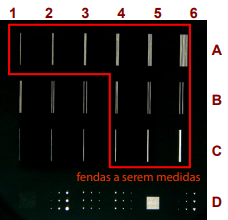
\includegraphics[scale=0.6]{figuras/rede_dif.png}
	\caption{Vidro e fendas utilizadas}
	\label{fig:rede}
\end{figure}

A fim de coletar os dados, buscando medir padrões de difração para fendas simples, o laser foi incidido na fenda C4, de forma que o padrão de difração pudesse ser observado em um papel milimetrado utilizado como anteparo. O procedimento foi repetido para as fendas C5 e C6.

Para esta situação, o modelo de difração de Fraunhofer~\cite{ref:otica} mostra que:
\begin{equation*}
    \Delta y \approx \frac{2 \lambda z}{b} \label{eq:difr}
\end{equation*}

Sendo que $\Delta y$ é a largura dos máximos da difração, $z$ a separação entre o emissor de luz e o anteparo e $\lambda$ o comprimento de onda da luz emitida. Com isso, dado que $z$ pode ser medido experimentalmente e conhecendo o comprimento de onda, é possível determinar a largura das fendas $b$, sendo este o procedimento realizado pelo grupo.

Na sequência, foram medidos os padrões para fendas duplas, B4, B5 e B6, e múltiplas, de A1 a A6, utilizando o mesmo procedimento anterior. Vale ressaltar que, para as fendas duplas, as espessuras eram iguais, enquanto, para as fendas múltiplas, as aberturas e as separações eram, nominalmente, as mesmas, mudando apenas o número de fendas.

Aplicando o modelo de Fraunhofer~\cite{ref:otica} sobre a interferência de fendas duplas, a separação entre máximos (ou mínimos) consecutivos no anteparo é dada por:
\begin{equation}
    \Lambda \approx \frac{\lambda z}{h} \label{eq:duplas}
\end{equation}

Onde que $h$ é a separação entre as fendas. Assim, de forma análoga ao processo para fendas simples, é possível determinar a separação entre as fendas a partir do comprimento de onda da luz emitida. Para determinação da largura das fendas, bastou aplicar o modelo de Fraunhofer para difração em fenda simples, já que para fendas duplas o fenômeno de difração também ocorre juntamente com interferência.

Já para uma quantidade generalizada $N$ de fendas, a análise muda e passamos a pensar na largura dos máximos primários $\delta\gamma$, que é aproximadamente metade da largura da base e é dada por:
\begin{equation}
    \delta y \approx \delta\gamma = \frac{\lambda z}{N h} \label{eq:mult}
\end{equation}

Em que $\delta y$ é a metade da largura da base dos máximos primários. Nota-se, também, que essa equação engloba o caso de fendas duplas, já que no caso específico de $N = 2$, teremos $\Lambda = 2 \delta y \approx 2 \frac{\lambda z}{2 h} = \lambda z / h$

As fendas múltiplas de mesma separação (A2-A6) também foram utilizadas para comprovar a relação: $$\delta y \propto \frac{1}{N} \label{rel:dyn}$$ Para tanto, montou-se um gráfico log-log de $\delta y \times N$ e, então, foi feita uma regressão linear do tipo $\log(\delta y) = A + B \log(N)$. Com essa regressão, $B$ se torna o expoente de $N$ na relação acima. A regressão foi seguindo o recomendado no Gui de Incertezas~\cite{ref:gum}, bem como as incertezas de cada coeficiente.

A próxima etapa do experimento consistia da observação de padrões de difração com a luz incidindo em um fio de cabelo, onde foi utilizado um pequeno quadro de material plástico, de tamanho similar ao vidro utilizado anteriormente, com o fio de cabelo fixado em seu centro (figura \ref{fig:fiocab}). A luz foi incidida no feixe e o padrão gerado foi observado no anteparo. É importante notar que, de acordo com o Princípio de Babinet~\cite{ref:wolf}, o modelo de Fraunhofer para fendas simples é aplicável para este padrão de difração, fazendo com que a determinação da largura do fio de cabelo seja análoga a determinação da largura de uma fenda simples.

\begin{figure}[H]
	\centering
	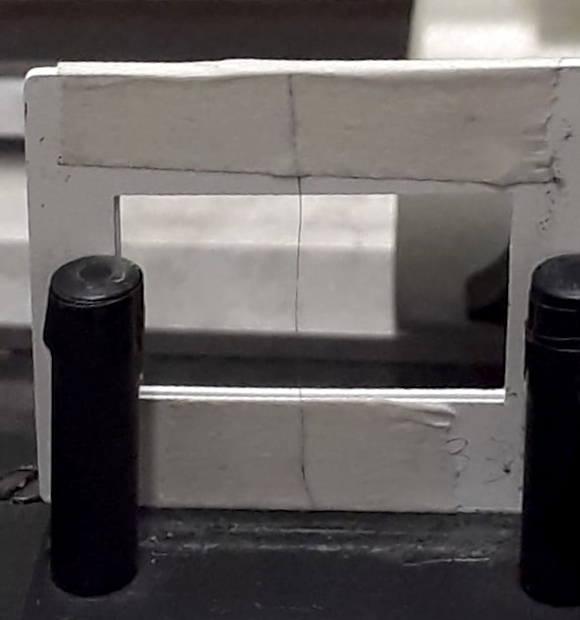
\includegraphics[scale=1.6]{figuras/mcabelo.jpg}
	\caption{Fio de cabelo utilizado}
	\label{fig:fiocab}
\end{figure}

A última etapa de observações foi feita analisando os padrões de difração em aberturas variadas, em geral, não sendo fendas. O mesmo procedimento citado anteriormente foi realizado para as aberturas D, com intuito de inferir o formato presente em cada uma.

Durante todos os procedimentos descritos anteriormente, fotos do anteparo foram tiradas utilizando um celular, a fim de analisar os padrões formados utilizando o \textit{software} \texttt{ImageJ}\cite{ref:imagej}. Assim possibilitando a determinação das distâncias dos mínimos de difração ($\Delta y$), dos máximos de interferência ($\Lambda$) e a largura da base dos máximos primários ($2 \delta y$). Além disso, o grupo determinou que a resolução do papel e a medição do distanciamento do anteparo foram as principais fontes de incerteza a serem consideradas. Vale citar que outras fontes de incerteza, como o posicionamento (paralaxe) e resolução da câmera também foram identificadas apesar de não serem consideradas durante o processamento dos dados, pois se tratavam de incertezas de difícil abordagem e buscou-se minimizá-las durante a coleta de dados.

Por fim, utilizando um microscópio metrológico, foram medidas as larguras das fendas ($b$), a separação entre elas ($h$) e a quantidade de fendas ($N$), em todas as situações anteriores. Também foram evitadas medições repetidas com esse equipamento, no caso, as separações e as larguras das fendas da linha A, que eram iguais. Para a utilização desse microscópio,foram identificadas como incertezas sua resolução e paralaxe na leitura.

\subsection{Incertezas}
    Começando pela incerteza das medidas de dimensão experimentais, no caso, a trena usada para medir a distância $z$ da fenda ao anteparo e o papel milimetrado. Como são medições analógicas, pode-se assumir uma ditribuição triangular, fazendo a incerteza da medição ser:
\begin{equation*}
    u_\text{medição} = \text{resolução} \times \frac{\sqrt{6}}{12}
\end{equation*}

Partindo disso, no caso da trena, assume-se uma incerteza de calibração, que seria como a incerteza de medição do ponto \SI{0}{\centi\meter}, isto é, $u_\text{calibração} = u_\text{medição}$. A incerteza total então seria:
\begin{align*}
    u_\text{total}
        &= \sqrt{u_\text{calibração}^2 + u_\text{medição}^2} \\
        &= u_\text{medição} \sqrt{2} \\
        &= \text{resolução} \times \frac{\sqrt{3}}{6}
\end{align*}

Já no caso do papel milimetrado no anteparo, esse tipo de incerteza não é aplicável, porém como a medição é dada por dois pontos, teremos duas incertezas $u_\text{medição}$, o que torna a incerteza total igual a da trena. Um ponto a expor sobre essa medida é que ela é encontrada a partir de duas dimensões, o que complica os cálculos da incerteza, porém, esse valor é encontrado pelo \texttt{ImageJ}\cite{ref:imagej}, onde o resultado é bem mais preciso, o que deixa válida a assunção de apenas a incerteza de medição de maneira linear.

Para ambos os casos acima $\text{resolução} = \SI{1}{\milli\meter}$, e, então, $u_\text{total} = \SI{.3}{\milli\meter}$. Dentre as medidas calculadas com isso, existe o $z$, que então fica $\Delta z = \SI{.3}{\milli\meter}$.

Agora, para os valores calculados, foram feitas as devidas propagações de incertezas, tendo como referência o padrão do INMETRO, o GUM\cite{ref:gum}. O primeiro desses valores é o $b$, da equação \ref{eq:difr}, cujas derivadas parciais são:
\begin{gather*}
    \frac{\partial b}{\partial z} = \frac{2 \lambda}{\Delta y} \\
    \frac{\partial b}{\partial \lambda} = \frac{2 z}{\Delta y} \\
    \frac{\partial b}{\partial (\Delta y)} = -\frac{2 \lambda z}{(\Delta y)^2}
\end{gather*}

Porém, como não não existe uma incerteza associada a $\lambda$, tem-se:
\begin{align*}
    \Delta b
        &= \sqrt{\left(\frac{\partial b}{\partial z}\right)^2 (\Delta z)^2 + \left(\frac{\partial b}{\partial (\Delta y)}\right)^2 (\Delta (\Delta y))^2} \\
        &= \frac{2 \lambda}{\Delta y} \sqrt{(\Delta z)^2 + z^2 \left(\frac{\Delta (\Delta y)}{\Delta y}\right)^2}
\end{align*}

Um passo importante para reduzir a incerteza numericamente, que também faz parte do procedimento do experimento, é o cálculo de $n_y$ larguras de máximo, em vez de apenas um. Assim, a medida passa a ser $n_y \Delta y$, com a mesma incerteza do $\Delta y$ original. A nova incerteza passar a ser:
\begin{equation*}
    \Delta (\Delta y) = \frac{\Delta (n_y \Delta y)}{n_y} = \frac{u_\text{total}}{n_y}
\end{equation*}

Com um proccesso bem similar aplicado na separação $h$ das fendas duplas, pela eq. \ref{eq:duplas}, chega-se em:
\begin{equation*}
    \Delta h = \frac{\lambda}{\Lambda} \sqrt{(\Delta z)^2 + z^2 \left(\frac{\Delta \Lambda}{\Lambda}\right)^2}
\end{equation*}

Aplicando o mesmo processo de redução da incerteza, isto é, medindo $n_\Lambda \Lambda$, no lugar de somente $\Lambda$, a incerteza reduz para $\Delta \Lambda = u_\text{total}/n_\Lambda$ também.

Para a separação de múltiplas fendas (eq. \ref{eq:mult}), a propagação é novamente muito similar, resultando em:
\begin{equation*}
    \Delta h = \frac{\lambda}{N \delta y} \sqrt{(\Delta z)^2 + z^2 \left(\frac{\Delta \delta y}{\delta y}\right)^2}
\end{equation*}

Nesse caso, no entanto, a redução de incerteza usada anteriormente não é aplicável.

Para a medida final, com o micrômetro metrológico, voltam as incertezas de medidas experimentais. A incerteza de leitura é parecido com a usada na trena, porém a incerteza de paralaxe, devido a leitura com a lupa, assume uma distribuição retangular, pois pode facilmente mudar a leitura uma casa acima ou abaixo, de acordo com a posição do observador. Assim:
\begin{gather*}
    u_{\text{medição}} = \frac{\text{resolução}}{2 \sqrt{6}} = \text{resolução} \times \frac{\sqrt{6}}{12} \\
    u_{\text{paralaxe}} = \frac{2\ \text{resolução}}{2 \sqrt{3}} = \text{resolução} \times \frac{\sqrt{3}}{3} \\
    \Delta L_i = u_{\text{total}}
        = \sqrt{u_{\text{medição}}^2 + u_{\text{paralaxe}}^2}
        = \text{resolução} \times \frac{\sqrt{6}}{4}
\end{gather*}

Então, como $b = L_2 - L_1$ e $h = L_3 - L_2$:
\begin{equation*}
    \Delta b = \Delta h = \sqrt{(\Delta L_i)^2 + (\Delta L_{i-1})^2} = u_\text{total} \sqrt{2} = \text{resolução} \times \frac{\sqrt{3}}{2}
\end{equation*}

Sendo que a resolução do equipamento é \SI{1}{\micro\meter}, a incerteza é $\Delta b = \Delta h = \SI{.9}{\micro\meter}$.

